\documentclass[11pt, a4paper]{article}
\setlength{\oddsidemargin}{0.5cm}
\setlength{\evensidemargin}{0.5cm}
\setlength{\topmargin}{-1.6cm}
\setlength{\leftmargin}{0.5cm}
\setlength{\rightmargin}{0.5cm}
\setlength{\textheight}{24.00cm} 
\setlength{\textwidth}{15.00cm}
\parindent 0pt
\parskip 5pt
\pagestyle{plain}

\newcommand{\namelistlabel}[1]{\mbox{#1}\hfil}
\newenvironment{namelist}[1]{%1
\begin{list}{}
    {
        \let\makelabel\namelistlabel
        \settowidth{\labelwidth}{#1}
        \setlength{\leftmargin}{1.1\labelwidth}
    }
  }{%1
\end{list}}

\usepackage{graphicx}
\graphicspath{ {../figs/} }
\usepackage{hyperref}
\usepackage{cite}

\begin{document}


\begin{namelist}{xxxxxxxxxxxx}
\item[{\bf Title:}]
    Learning Automata of Black Box Software and Hardware with Side Channel Analysis
\item[{\bf Author:}]
	Johnathan DiMatteo
\item[{\bf Supervisor:}]
	Sebastian Fischmeister
\end{namelist}

\section*{Motivation}
% In this section you should give some background to your
% research area. What is the problem you are tackling, and why is it
% worthwhile solving? Who has already done some work in this area,
% and what have they achieved?
How do we verify software systems are properly designed and secure?
One way is to create a \textit{model} of the software to compare to the specifications.
There are numerous ways to infer models by analyzing code or performing tests (such as black box fuzzing).
Black box fuzzing sends random or malformed input to a system to get the system to crash or respond in a way that does not conform to specifications.
The goal is to ensure a completed system does not have unintended behaviour, which could ultimately lead to vulnerabilities.
But \textit{model learning}, also known as automata learning, is about algorithms that are able to learn a complete representation of software systems automatically.
Similar to how humans learn, the algorithms provide inputs and observe outputs to determine the global states of the system.
They use past behaviour of the system to select the next input to send.
Over time, they can identify valid transitions and which states the system should be in to build an accurate representation (such as a state diagram or other) of the software system.
With this representation, vulnerabilities should be easy to spot.
Some examples of case studies where vulnerabilities were identified using model learning are: Transport Layer Security (TLS) protocols \cite{TLS}, Windows 8 TCP Client \cite{fiteruau2016combining}, and credit card readers \cite{chalupar2014automated}. 
As more and more companies are adopting and using IoT devices, this has become an extremely important research topic to ensure software and hardware systems conform to specifications and work as intended.

The goal of this paper is to enforce security and safety in devices through \textit{Model Learning}.
% ============= MODEL LEARNING ===============%
Our proposed method is to use \textit{Side Channel Analysis} to make learning more ``black box''.

\subsection*{Background}

\textbf{State diagrams} are a way to model a system concerning a finite number of states, inputs and outputs.
\textbf{Inputs} are external stimuli that interact with the system.
\textbf{Outputs} are a system's response to an input.
%============== WHAT IS A STATE? COFFEE MACHINE EXAMPLE ====== %
A \textbf{state} determines the behavior of a system.
For example, a coffee machine can have three states, ``Off'', ``Standby'', and ``Ready''.
The coffee maker will only pour coffee after the press of Button B in the ``Ready'' state, will be turned off in the ``Off'' state, and will wait for the user to load a coffee pod in the ``Standby'' state.
A state is bound to a set of rules and functions (i.e. it is impossible to pour coffee in the ``Off'' state).
State diagrams are common in software validation.
We will be focusing on a specific type of state diagram model known as a Mealy Machine.

%======WHAT IS A STATE DIAGRAM MODEL ========%
% ======= INPUTS? OUTPUTS? ===== %

%\begin{figure}[!h]
%    \hspace*{2cm}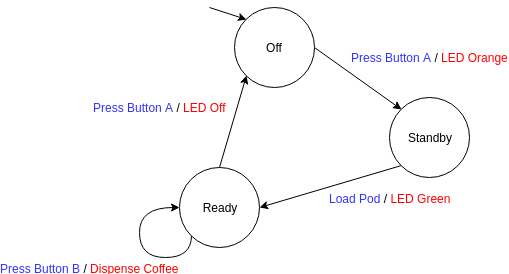
\includegraphics[scale=0.5]{coffee}
%    \caption{Example of a simple Mealy Machine for a coffee maker.}
%    \label{coffee}
%\end{figure}
\begin{figure}
    \centering
    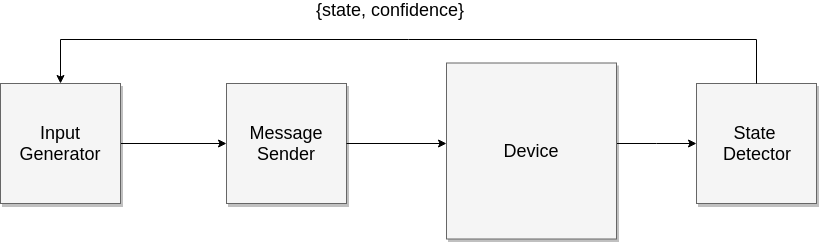
\includegraphics[scale=0.5]{state-detector.png}
    \label{The system under active model learning.}
\end{figure}

\section*{Problem Statement} 
%Now state explicitly the hypothesis you aim to
%test. Make references to the items listed in the Reference section
%that back up your arguments for why this is a reasonable
%hypothesis to test, for example the work of Knuth~\cite{knuth}.
%Explain what you expect will be accomplished by undertaking this
%particular project.  Moreover, is it likely to have any other
%applications?

\begin{enumerate}
    \item \textbf{Input Generator}: Given the current predicted state (\textbf{output? - ask Sebastian}) and history of previous states (\textbf{outputs?}) and queries, determine the next query that is most likely to induce a state change in the system under observation.
    \item \textbf{State Detector}: Given a response from the system under observation and history of previous responses, estimate the current state (\textbf{output? - ask Sebastian}).
    \item \textbf{Message Sender}: Given a query, translate the query into a valid message accepted by the system.
    %valid inputs to system and outputs from the system to valid inputs to the Learner.
    %the Learner's queries into valid inputs to the system, 
    %and classifying the response of the system to the output alphabet understood by the Learner.
\end{enumerate}

\nocite*{}
\bibliography{bibfile}{}
\bibliographystyle{plain}

\end{document}


